\documentclass[11pt]{article}
\usepackage{amsmath, amssymb, amsthm}
\usepackage{geometry}
\usepackage{graphicx}
\usepackage{hyperref}
\usepackage[backend=biber]{biblatex}
\addbibresource{../references.bib}
\geometry{margin=1in}
\title{Informational Equivalence and Entropy Collapse in Black Hole Simulation}
\author{Juha Meskanen}
\date{2024}

\begin{document}
\maketitle


\begin{abstract}
  Building on our earlier proposal that the universe is fundamentally informational in nature, we present a computational model of black hole singularities based on the entropy of execution traces. By simulating black hole evolution as a computational process, we represent system states as bitstrings and define a mapping from information to spacetime geometry. We show that vanishing Shannon entropy corresponds to geometric collapse into a singular point in any embedding space. A Python simulation illustrates this entropy–geometry correspondence in dynamic systems. This supports the view that geometric singularities may emerge from informational degeneracy.
\end{abstract}

\section{Introduction}

This paper builds on a previously proposed framework in which physical reality, including time and conscious experience, emerges from information encoded in formal axiomatic systems \cite{meskanen2019}. In that model, systems like human beings and their digital simulations are viewed as different realizations of the same informational content. Extending this principle, we now explore whether a black hole—a classically continuous geometric object—can also be represented as an informational system. Specifically, we ask: if the universe is fundamentally discrete and informational, what does a black hole singularity look like under this ontology?


This leads to a central claim:

\begin{quote}
  \textbf{Lemma (Entropy--Singularity Lemma):} \emph{Vanishing entropy implies geometric singularity.}
\end{quote}

The paper is structured as follows: we first define the program execution trace using set theory, then describe how such traces map to discrete representations of spacetime. We formalize and defend the lemma and explore its physical consequences.

\section{Methods}

We model the evolution of a black hole spacetime geometry as a set of bitstrings encoding the information in the spacetime. This is accomplished as a simulation where the memory image encoding the spacetime geometry is traced and represented as an ordered set of bitstrings. Even though the simulation cannot be run to  completion due to  fundamental limits and numerical precision, we can analyze the evolution of the bitstrings and extrapolate the simulation to completion using statistical methods. As the simulation
models the qualitative behavior of the black hole, we hope to gain insight into the nature of black hole singularities and their relationship to entropy.
The simulation is implemented in Python, and the source code is available at \url{http://githumb/juhakm/Schwarzschild\_entropy.py}.


\section{Execution Trace in Set-Theoretic Form}

Let $\mathcal{M}$ be the set of all addressable memory units in a machine. Each machine state $s \subseteq \mathcal{M}$ is a subset containing the values of all memory units, registers, and CPU state.

Define $S$ as the set of all possible machine states. Let a program be a finite sequence of instructions:
\[
  P = (I_1, I_2, \dots, I_n)
\]
Each instruction $I_i$ defines a transition function $I_i : S \to S$.

We define the execution trace as an ordered superset of visited states:
\[
  T = (s_0, s_1, \dots, s_n) \quad \text{where } s_{i+1} = I_{i+1}(s_i)
\]

The associated transition relation induced by $P$ is:
\[
  R_P = \{ (s_i, s_{i+1}) \in S \times S \mid s_{i+1} = I_{i+1}(s_i) \}
\]

\section{Mapping Information to Spacetime Geometry}

We represent points in 3D space as triples of integers:
\[
  (x_1, x_2, x_3) \in \mathbb{Z}^3
\]
Each coordinate is derived from a fixed-width binary encoding of simulation data.

Let $b \in \{0,1\}^L$ be a bitstring encoding the complete system state. Let:
\[
  \mathcal{C} = \{0,1\}^{3k}
\]
be the configuration space representing all geometric states under $3k$ bits. Define a mapping:
\[
  f : \mathcal{C} \to \mathbb{Z}^3, \quad f(b) = (\phi(b_1), \phi(b_2), \phi(b_3))
\]
where $\phi : \{0,1\}^k \to \mathbb{Z}$ decodes binary segments.

\section{Entropy Collapse and Geometric Singularity}

Define the empirical frequency $p_T(s)$ over the execution trace $T$:
\[
  H(T) = -\sum_{s \in T} p_T(s) \log_2 p_T(s)
\]

If $H(T) \to 0$, the system visits a single state repeatedly. Any geometric mapping applied to such a system collapses to a single point.

\begin{quote}
  \textbf{Lemma (Entropy--Singularity Lemma):}
  \emph{As Shannon entropy approaches zero, any mapping of informational states to geometric space collapses to a degenerate spatial representation — a pointlike structure — regardless of the coordinate system.}
\end{quote}


\begin{figure}[h!]
  \centering
  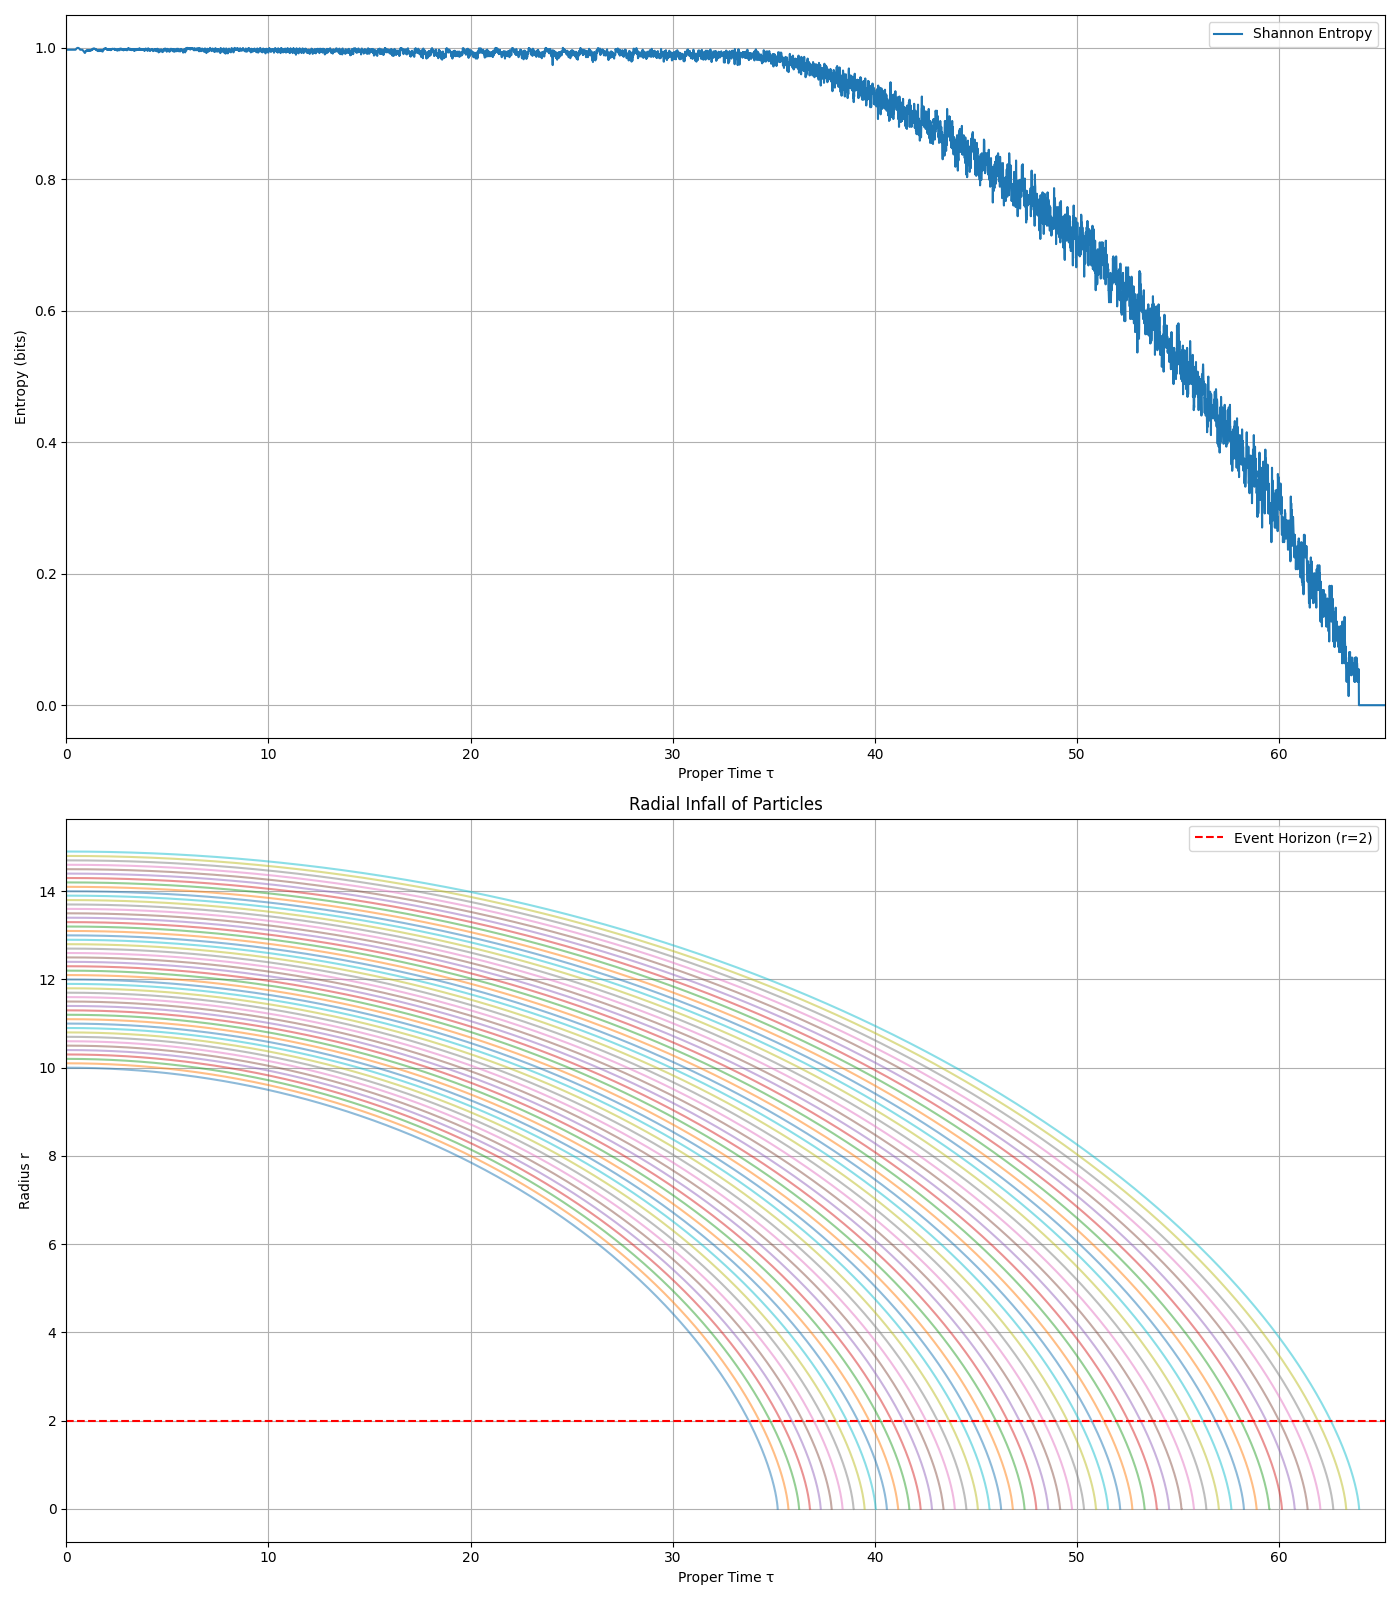
\includegraphics[width=1.0\textwidth]{figures/schwarzschild_entropy_signature.png}
  \caption{Particles falling in Schwarzschild metrics and the corresponding entropy signature of the execution trace. The entropy decreases as the particles approach the singularity, indicating a collapse of information into a point. By extrapolating the entropy signature, we can run the simulation to completion and analyze the properties of the singularity.
      [simulation program \url{http://github.com/juhakm/schwarzschild_entropy.py}]}
  \label{fig:vanishing_entropy}
\end{figure}



\subsection*{Justification}

This result does not depend on the specific method used to interpret a bitstring geometrically. When mapped to geometric representations---whether through integer decoding, floating-point interpretation, or structured coordinate systems---the lack of informational variability ensures that all resulting points coincide. The outcome is thus a pointlike structure in any embedding space. We regard this self evident.



\section{Simulation Details}

\begin{figure}[h!]
  \centering
  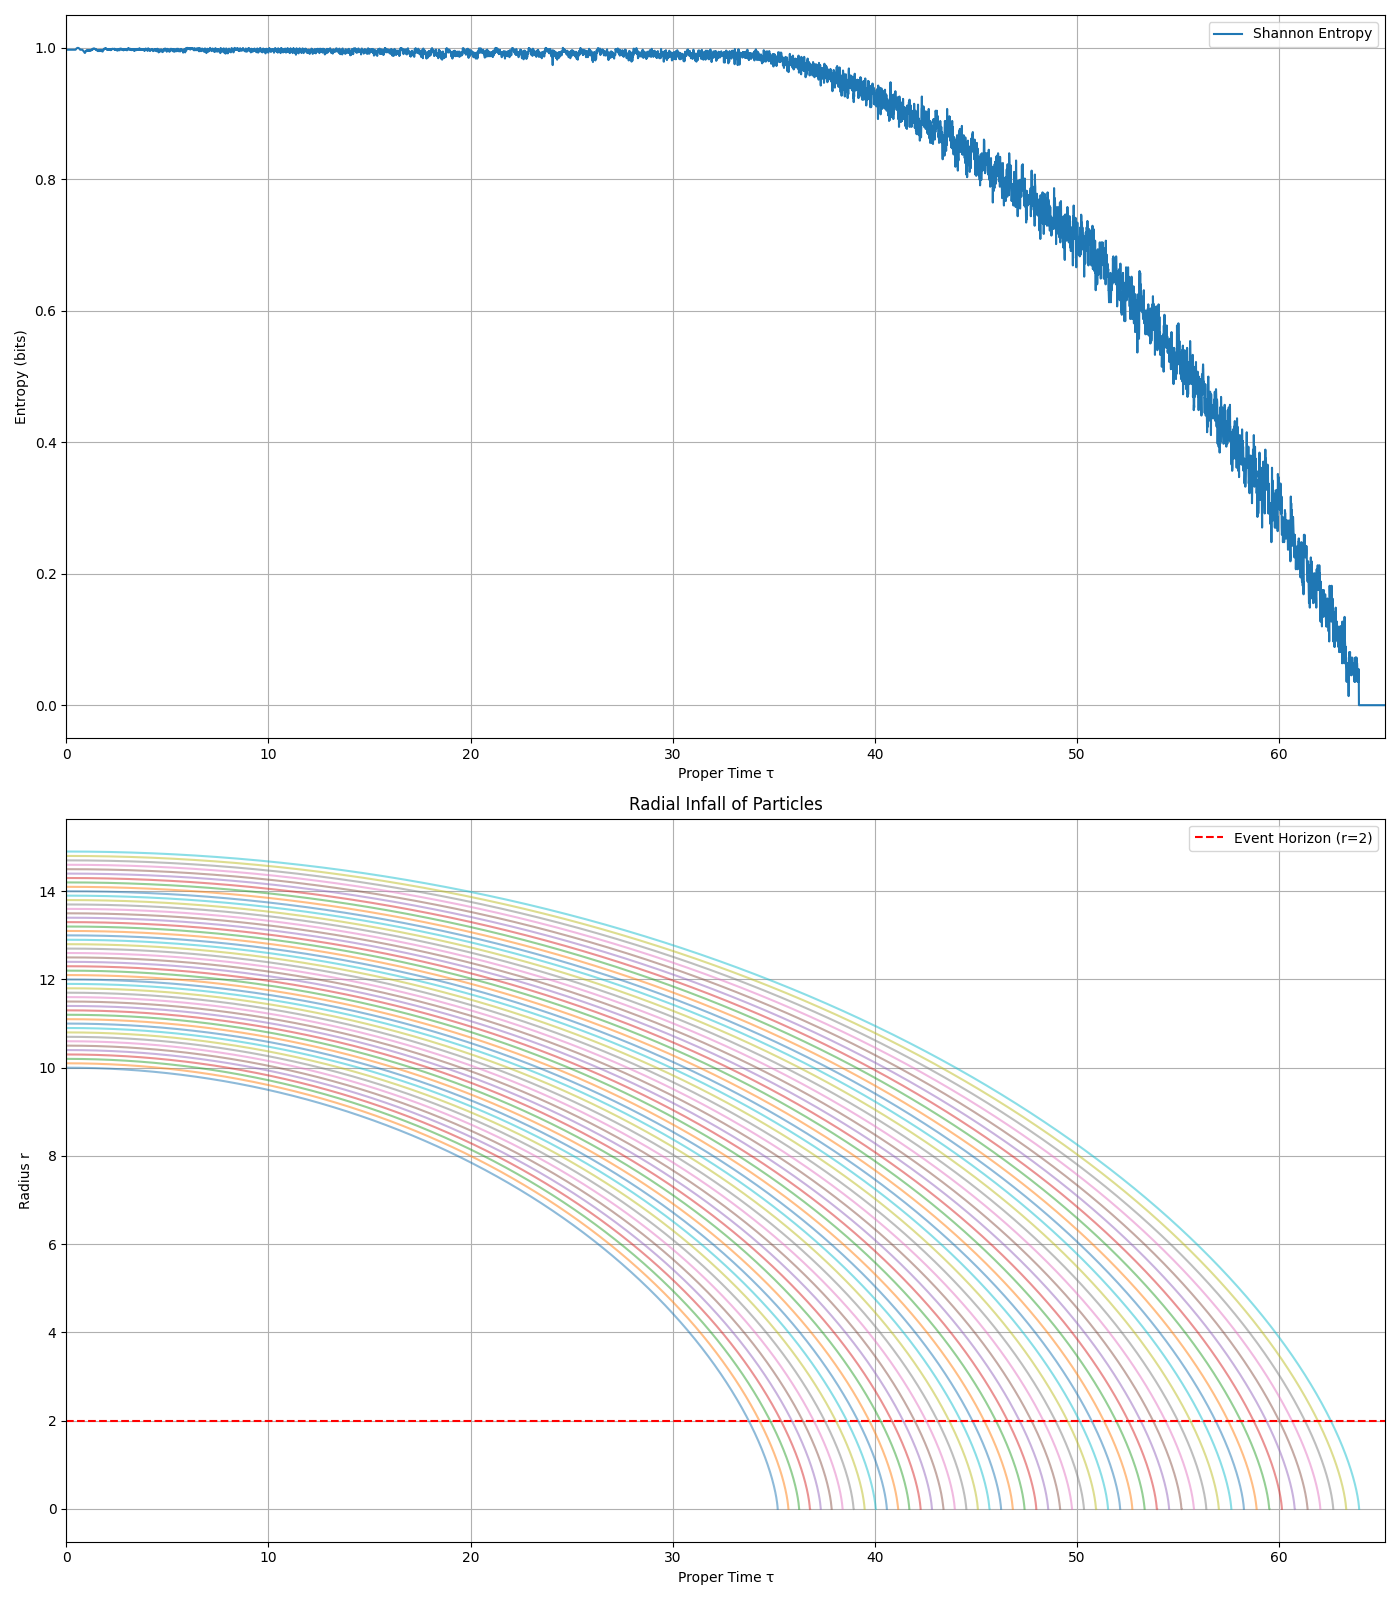
\includegraphics[width=1.0\textwidth]{figures/schwarzschild_entropy_signature.png}
  \caption{Particles falling in Schwarzschild metrics and the corresponding entropy signature of the execution trace. The entropy decreases as the particles approach the singularity, indicating a collapse of information into a point. By extrapolating the entropy signature, we can run the simulation to completion and analyze the properties of the singularity.
      [simulation program \url{http://github.com/juhakm/schwarzschild_entropy.py}]}
  \label{fig:vanishing_entropy}
\end{figure}




We implemented a Python simulation of a collapsing dust cloud. State data was quantized, serialized into bitstrings, and entropy was measured. Over time, bitstring entropy decreased, visually collapsing geometry into a point.

\begin{figure}[h!]
  \centering
  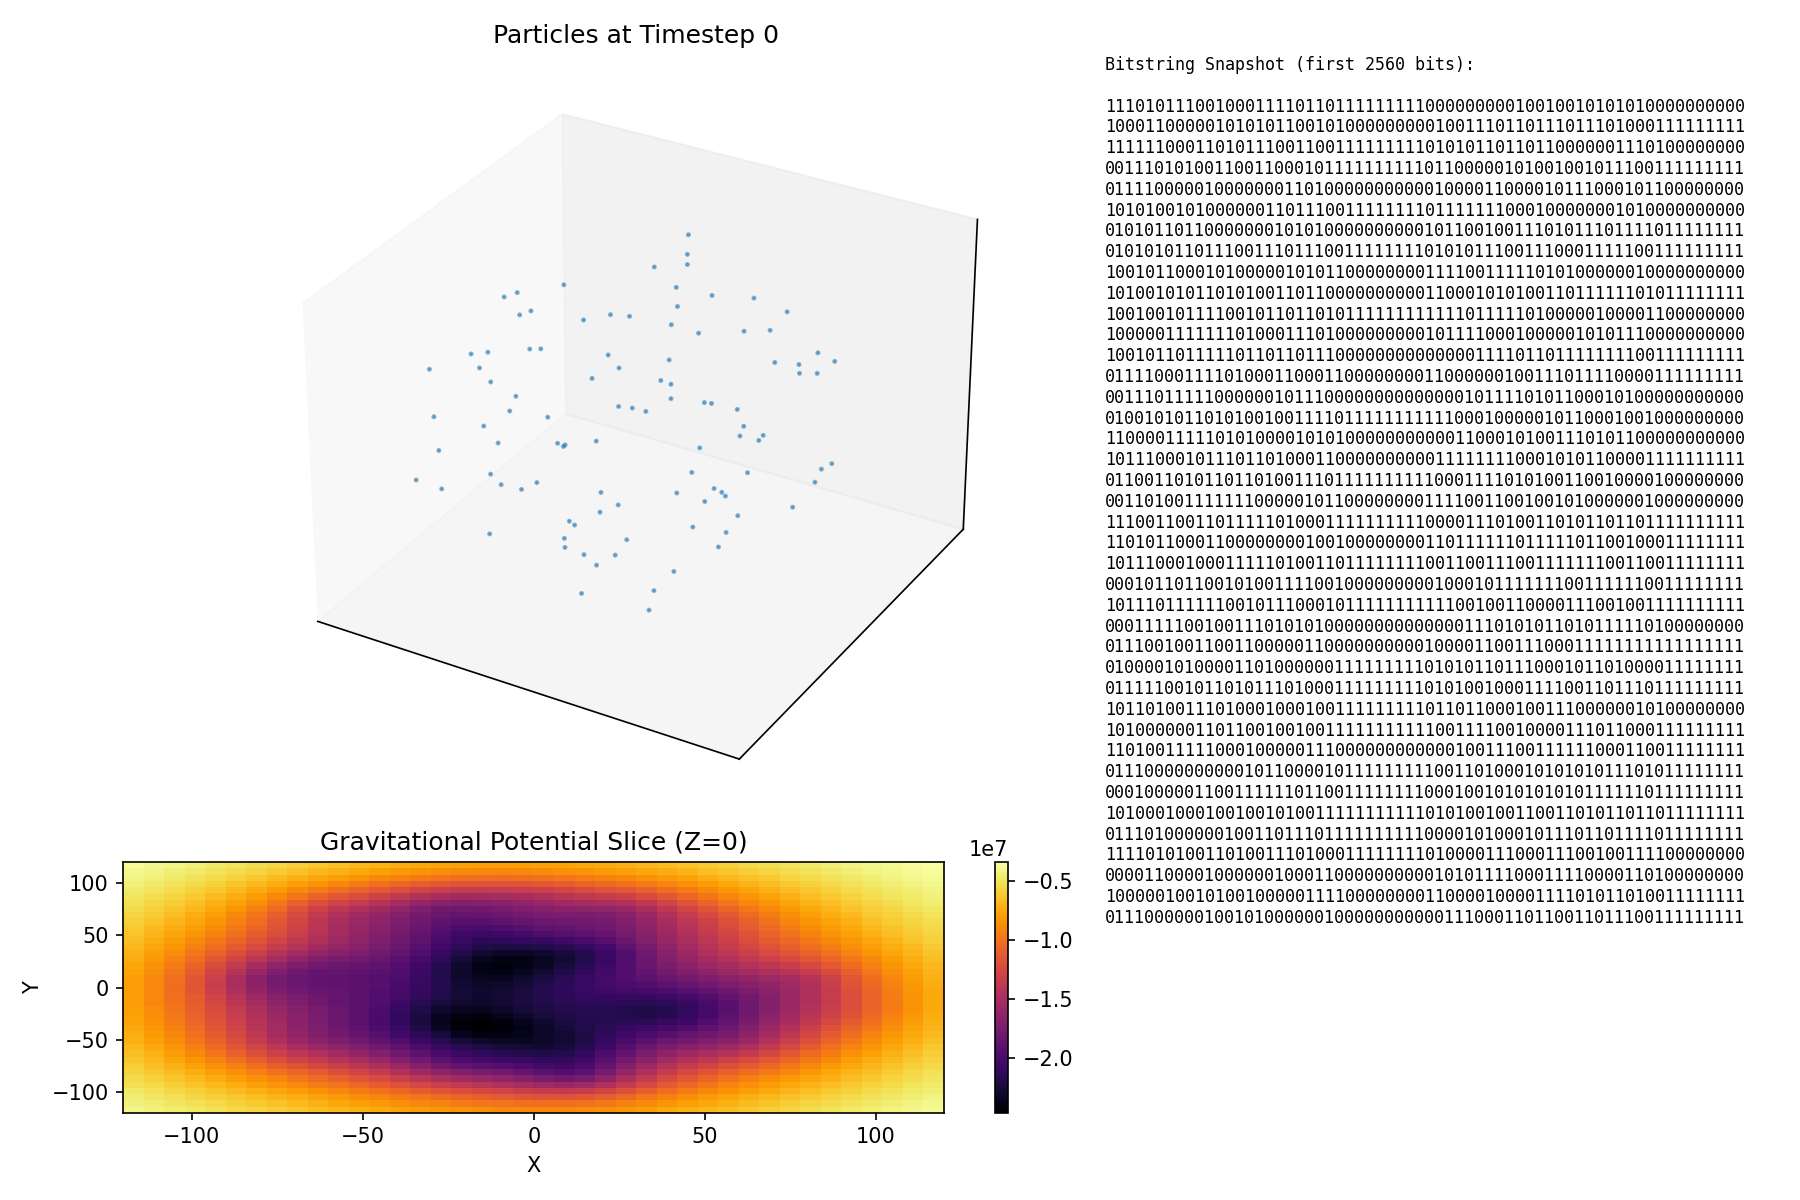
\includegraphics[width=1.0\textwidth]{figures/collapse_0.png}
  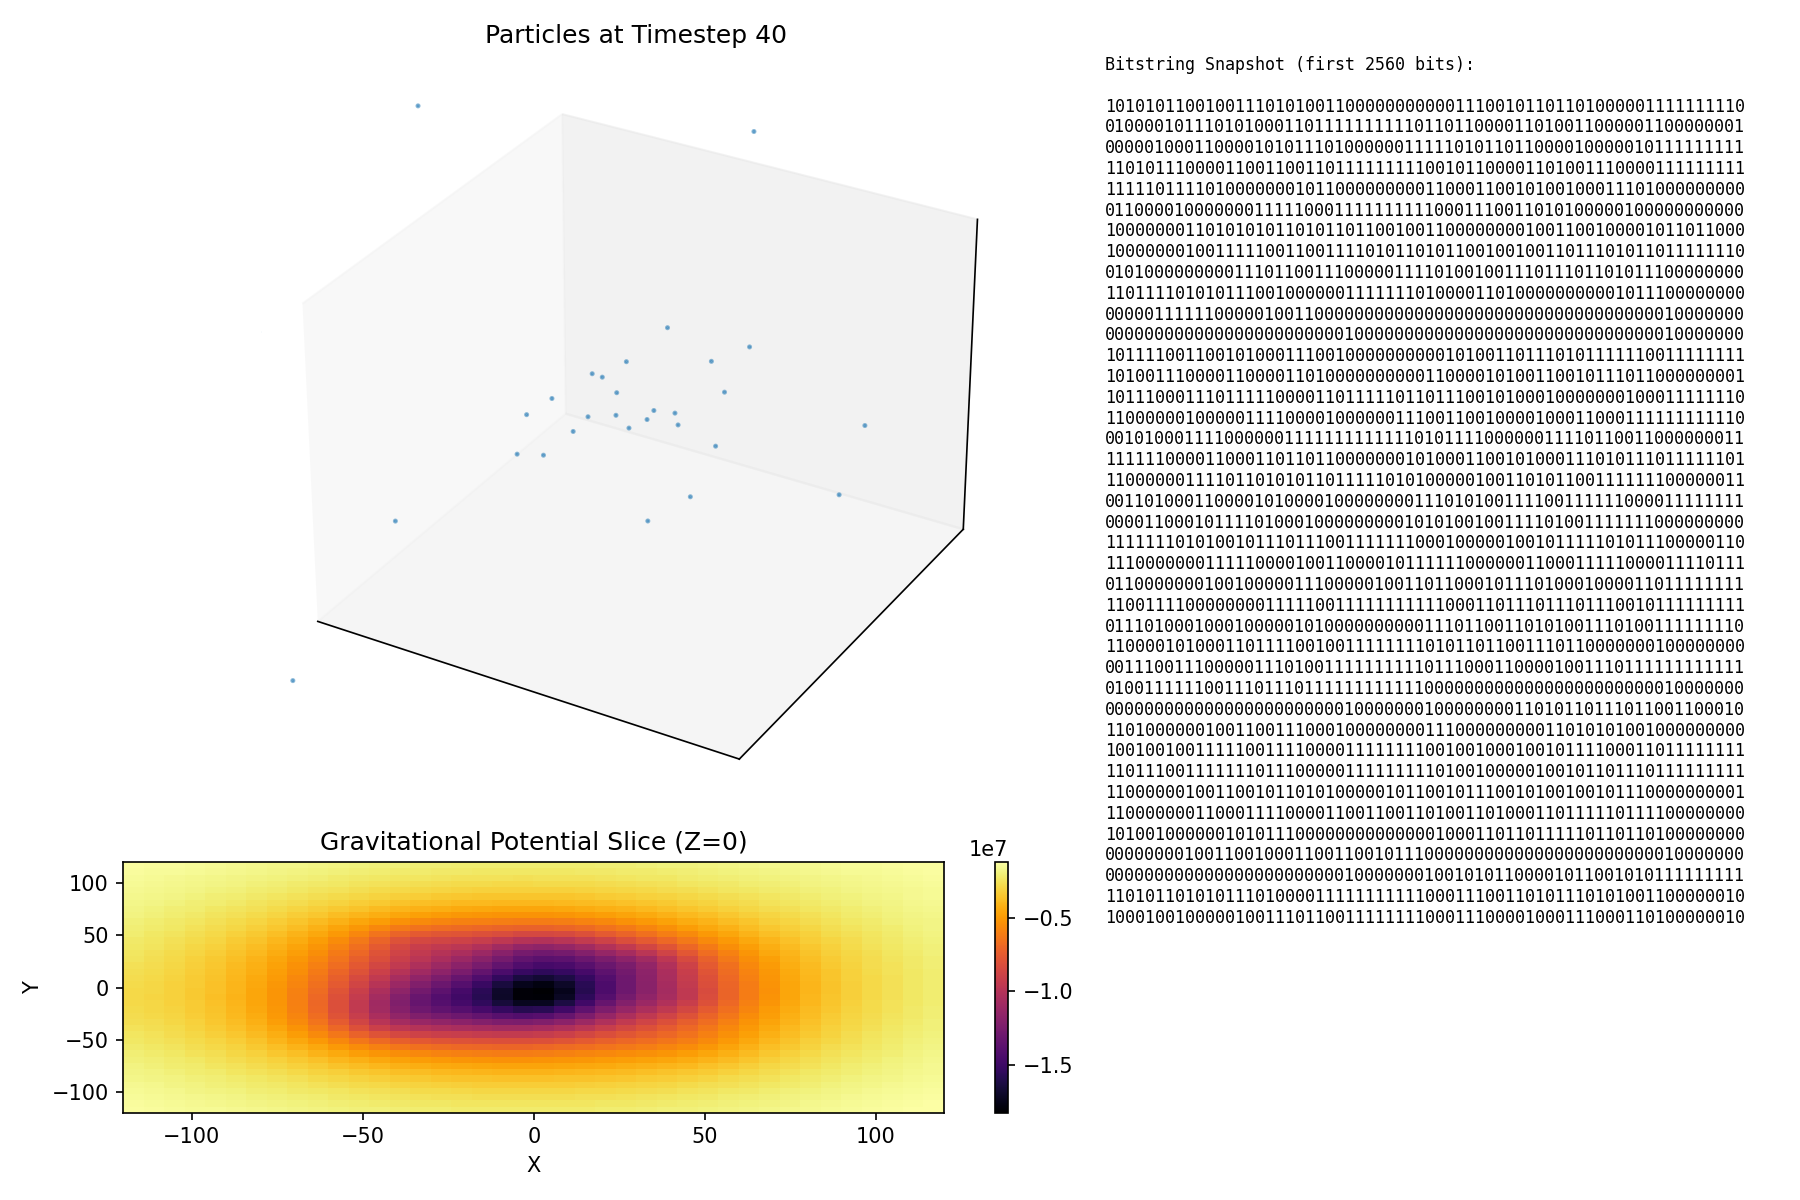
\includegraphics[width=1.0\textwidth]{figures/collapse_40.png}
  \caption{Collapsing spacetime geometry. As entropy decreases, spacetime collapses toward a point.}
  \label{fig:vanishing_entropy}
\end{figure}

\section{Conclusion and Future Work}

While the total entropy of the blackhole increases in accordance with the second law of thermodynamics, the entropy of the geometric encoding of a gravitationally collapsing system may decrease. This reflects increasing determinism and reduced configurational freedom as spacetime compresses. In this view, the region near the singularity becomes representable by an informationally degenerate structure—a bitstring of minimal entropy. Our simulation captures this local collapse of geometric entropy, not a reversal of thermodynamic law.

We have shown that zero-entropy informational states necessarily correspond to geometric singularities. This creates an absolute informational scale for entropy, anchored at zero. Future work will model entropy increase as emergent spacetime expansion, simulate structure formation, and explore whether entropy acts as a driver of geometric complexity.

\appendix
\section{Appendix: Bitstring Encoding}

\begin{itemize}
  \item Quantize floating point: $\mathbb{R} \to \mathbb{Z}$
  \item Serialize integers to binary
  \item Concatenate to $b \in \{0,1\}^L$
\end{itemize}

Entropy of $b$:
\[
  H(b) = -p_0 \log_2 p_0 - p_1 \log_2 p_1
\]
where $p_0$, $p_1$ are empirical frequencies.

\section*{References}
\begin{thebibliography}{9}
  \bibitem{Bekenstein1973} J. D. Bekenstein, "Black Holes and Entropy," \textit{Phys. Rev. D} \textbf{7}, 2333 (1973).
  \bibitem{Hawking1975} S. W. Hawking, "Particle Creation by Black Holes," \textit{Commun. Math. Phys.} \textbf{43}, 199 (1975).
\end{thebibliography}

\end{document}
